
Two cross-checks have been performed for Fill 7358 to understand if the systematic change in the slope values as a function of bcid are due to the afterglow corrections.
In the first check (Fig~\ref{fig:fill7358trainslope_crosscheckPCC}) the PCC afterglow corrections are removed, in the second check (Fig~\ref{fig:fill7358trainslope_crosscheckHFOC}) the HFOC residual afterglow corrections are removed.
In both tests the y-intercept values change, but the systematic trend on the slope values remains.

\vspace{36pt}
\begin{figure}[hc]
  \begin{center}
    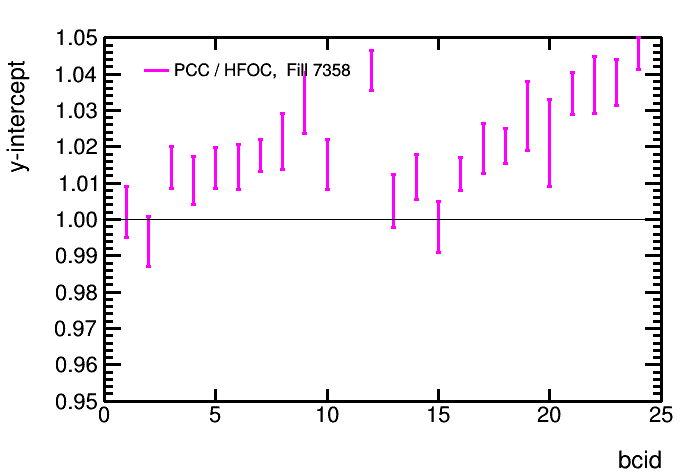
\includegraphics[width=0.47\linewidth]{plots/sbilratios_trains_Fill7358/plot_det_linearity_perbx_y0_7358_NoPCCCorr.png}
    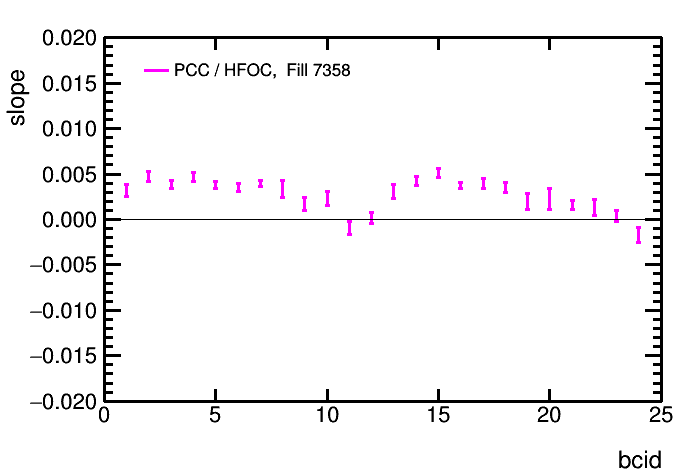
\includegraphics[width=0.47\linewidth]{plots/sbilratios_trains_Fill7358/plot_det_linearity_perbx_slope_7358_NoPCCCorr.png}
    \caption{
      y-intercept and slope values obtained from the linearity fits for the 24 bunches in the two trains of Fill 7358 after removing the PCC afterglow corrections.
      \label{fig:fill7358trainslope_crosscheckPCC}
    }

    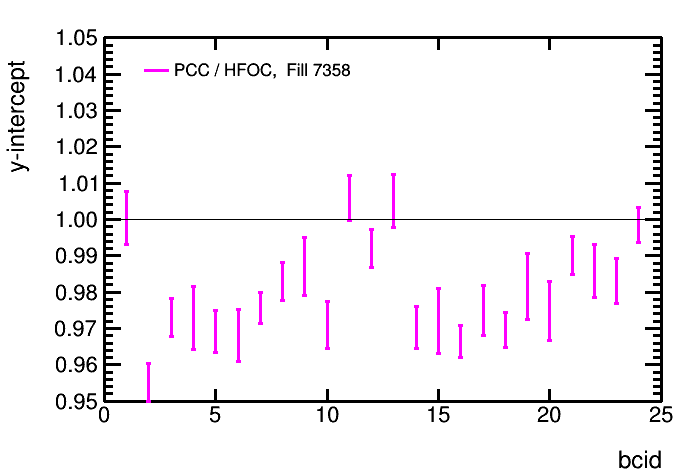
\includegraphics[width=0.47\linewidth]{plots/sbilratios_trains_Fill7358/plot_det_linearity_perbx_y0_7358_NoHFCorr.png}
    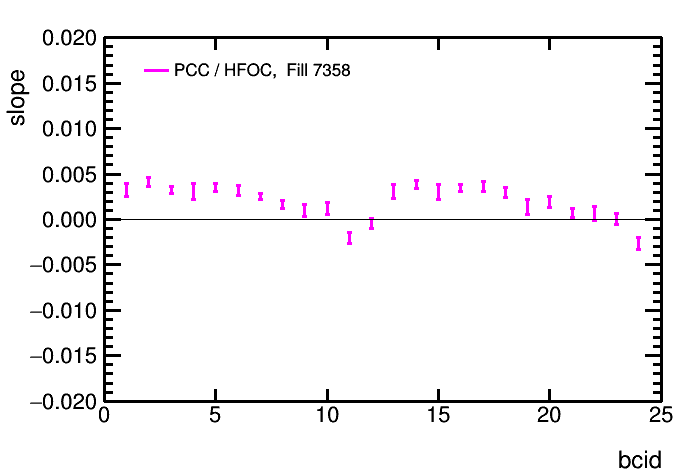
\includegraphics[width=0.47\linewidth]{plots/sbilratios_trains_Fill7358/plot_det_linearity_perbx_slope_7358_NoHFCorr.png}
    \caption{
      y-intercept and slope values obtained from the linearity fits for the 24 bunches in the two trains of Fill 7358 after removing the HFOC residual afterglow corrections.
      \label{fig:fill7358trainslope_crosscheckHFOC}
    }

  \end{center}
\end{figure}


%\begin{figure}[hb]
%  \begin{center}
%  \end{center}
%\end{figure}
%
